\chapter{ENet}
Later in our review of literature published related to segmentation models, we came across ENet (Efficient Neural Network), which is termed as a real-time semantic segmentation neural network designed for efficient processing on embedded systems and mobile devices. It was developed by researchers at Samsung AI Center and first presented in the paper "ENet: A Deep Neural Network Architecture for Real-Time Semantic Segmentation" published in 2016 [6].

Reviewing the research paper of ENet, it was found that performance wise and efficiency wise it is better than SegNet [5].

\begin{table}[h!]
    \centering
    \setlength{\arrayrulewidth}{0.5mm}
    \setlength{\tabcolsep}{18pt}
    \renewcommand{\arraystretch}{1.5}
    \begin{tabular}{ |p{1.5cm}|p{1.8cm}|p{1.8cm}|p{2cm}|p{2cm}| }
        % \hline
        % \multicolumn{5}{|c|}{Country List} \\
        \hline
        Network & 1024x512 & 1280x720 & Parameters & Model Size \\
        \hline
        ENet    & 20.4 ms  & 32.9 ms  & 0.36 M     & 1.5 MB     \\
        \hline
        SegNet  & 66.5 ms  & 114.3 ms & 29.4 M     & 117.8 MB   \\
        \hline
    \end{tabular}
    \caption{A comparison of computational time, number of parameters and model size required for ENet and SegNet [5]}
    \label{table:1}
\end{table}

The key advantages of ENet are its high speed, low computational requirements, and smaller memory footprint compared to existing models, while maintaining comparable accuracy. Considering the viability of the model for our project which mainly focuses on deploying a reliable model to identify boxes in an industrial environment, a suggestion was made at a discussion with the supervisor to consider this model, as it would allow us to deploy such a model in edge environments where memory and process is a constrained resource. The suggestion was reviewed and approved by the supervisor later and it lead to the transition from SegNet to ENet.

\subsection{Network Architecture}
The ENet architecture follows an encoder-decoder style topology with repeated modules of main and lateral branches. The encoder path captures higher-level semantics through a sequence of pooling and convolution operations, while the lateral connections preserve spatial information from earlier stages. The core building blocks are bottleneck modules with varying complexities [5]:

\begin{figure}[H]
    \begin{minipage}[t]{7.2cm}
        \begin{center}
            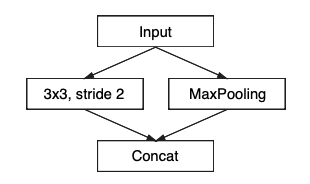
\includegraphics[width=200pt]{assets/enet/first.png}
            \caption{ENet initial block}
            \label{fig:using:enetinit}
        \end{center}
    \end{minipage}
    \hfill
    \begin{minipage}[t]{7.2cm}
        \begin{center}
            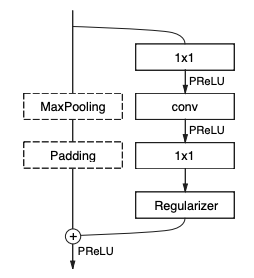
\includegraphics[width=200pt]{assets/enet/second.png}
            \caption{ENet bottleneck module}
            \label{fig:using:enetbottle}
        \end{center}
    \end{minipage}
\end{figure}

The following implementation in Pytorch achieves the network architecture provided by the paper [4]
\begin{description}
    \item[Initial Block:] Combines max-pooling and projection paths
    \item[Regular Bottleneck:] Applies identity mappings and 1x1 projections
    \item[Downsampling Bottleneck:] Reduces spatial dimensions with striding.
    \item[Dilated Bottleneck:] Employs dilated convolutions to expand receptive fields.
    \item[Upsampling Bottleneck:] Bilinear upsampling and fusion of encoder features.
\end{description}
This highly efficient architecture allows ENet to achieve real-time inference speeds while maintaining accuracy comparable to larger models like SegNet.

\section{Model Transition Plan 13/03/2024}
The following were planned to be acted on to create a model based on the original paper on ENet.
\begin{enumerate}
    \item Obtain the datasets mentioned in the paper (Cityscapes, CamVid, SUN RGB-D) and prepare them for training and testing.
    \item Implement the ENet architecture as described in the paper, including the encoder, decoder, and bottleneck modules. Using deep learning framework PyTorch
    \item Apply the design choices mentioned in the paper, such as early down-sampling, dilated convolutions, and Spatial Dropout.
    \item Train the ENet model on the datasets using the Adam optimization algorithm and the custom class weighing scheme described in the paper.
    \item Evaluate the trained model's performance on the test sets of the datasets, using metrics like class average accuracy, mean Intersection over Union (IoU), and inference time.
    \item Compare the results with existing models like SegNet, as done in the paper, and analyze the trade-offs between accuracy and processing time.
    \item Optionally, run the trained ENet model on embedded devices like the NVIDIA Jetson TX1 to assess its real-time performance and resource requirements.
\end{enumerate}

\section{ENet Paper Implementation 23/03/2024}
Paper implementation of ENet on CamVid dataset [4]. This guide assumes basic familiarity with notebooks and will include a brief setup process to get started with Google Colab.
\subsection*{Notebook Environment Setup: Google Colab}
\begin{enumerate}
    \item Go to \url{colab.research.google.com} -> File -> Open Notebook -> Search for the notebook from the Github Repo \url{https://github.com/CV-bin-picking/enet} and open it.
          \begin{figure}[H]
              \centering
              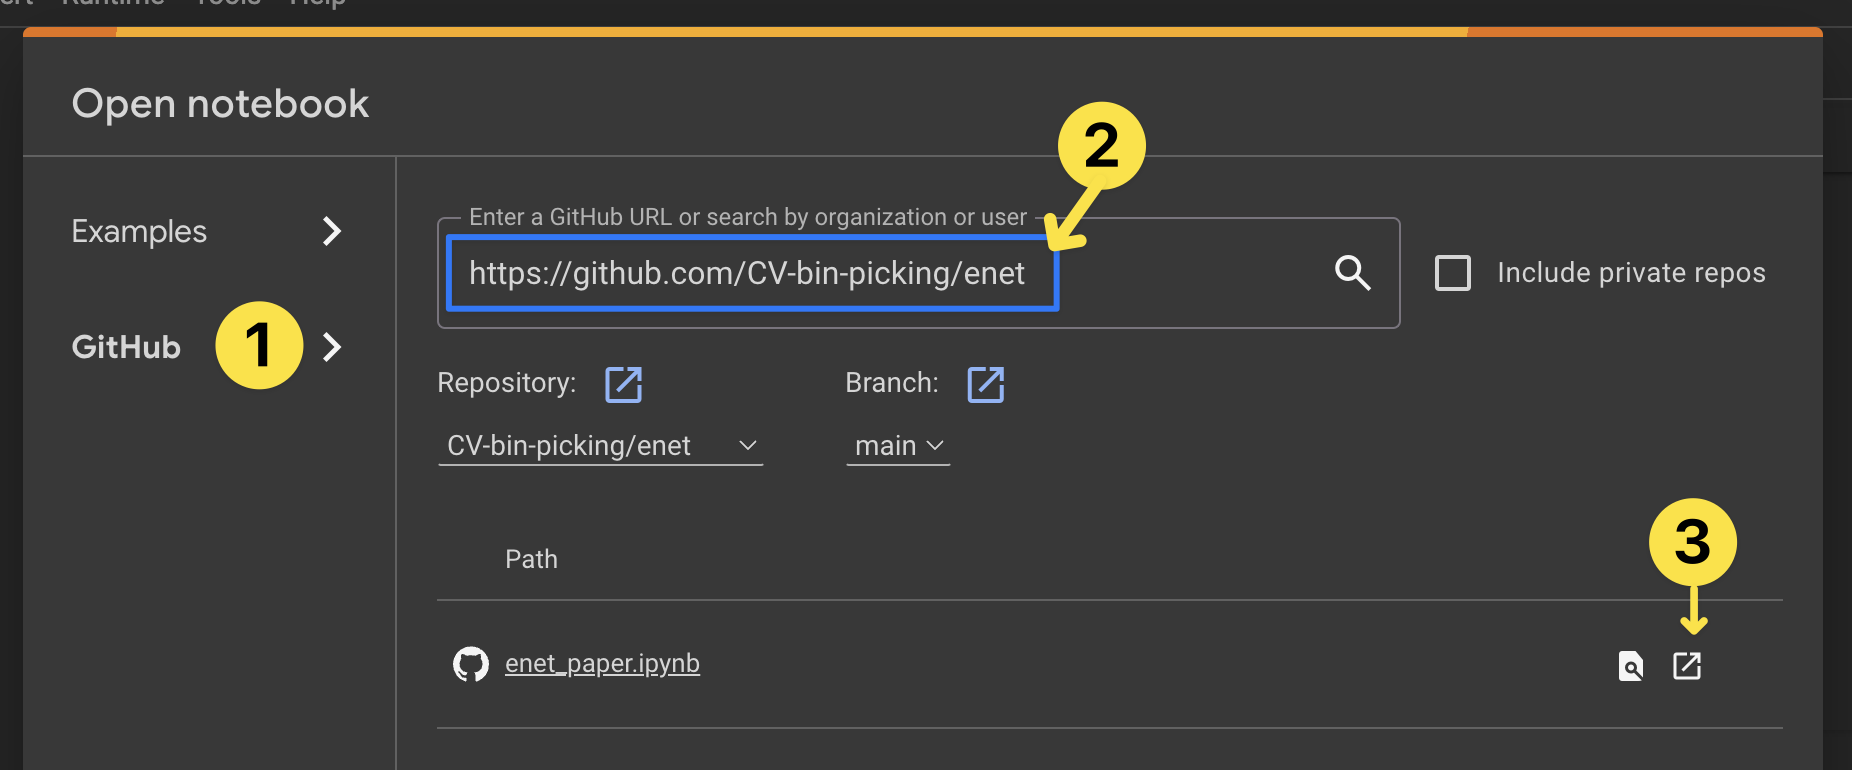
\includegraphics[width=450pt]{assets/enet/camvid/open.png}
              % \caption{SegNet Architecture Diagram}
              \label{fig:using:test1}
          \end{figure}
    \item Connect to GPU Runtime: In the menubar, go to Runtime -> Change runtime type. In the pop-up window, Runtime type as Python -> Select T4 GPU as the hardware accelerator -> Click Save.

          \textit{A Google Account is required. Colab interface is constantly changing, and it will autodetect recommended configurations for the notebook at launch. User is expected to do the best in either cases as GPU will improve the training time dramatically.}
    \item Importing dependencies: Execute the first cell in the notebook to prepare the python environment by importing required dependencies. \textit{You can ignore the warning about the notebook being not authored by Google after you've reviewed the source code}
          \begin{lstlisting}[language=Python]
import torch
import torch.nn as nn
import torch.nn.functional as F
import numpy as np
import matplotlib.pyplot as plt
from torch.optim.lr_scheduler import StepLR
import cv2
import os
from tqdm import tqdm
from PIL import Image
        \end{lstlisting}
    \item Configuring root directory: Change the root\_path variable string to "/content" before executing the second cell. This will configure the root directory where the model searches for the dataset and dumps the trained models. \textit{This step is allows the program to be executed in Colab as well as locally in your python environment with appropriate configuration.}
          \begin{lstlisting}[language=Python]
root_path = "/content" # change to `/content` for google colab
        \end{lstlisting}
    \item Configuring CamVid dataset: Uncomment the code in the third cell and execute it to download the CamVid dataset and extract it in the Colab root directory.
          \begin{lstlisting}[language=Python]
!wget https://www.dropbox.com/s/pxcz2wdz04zxocq/CamVid.zip?dl=1 -O CamVid.zip
!unzip CamVid.zip
        \end{lstlisting}
          \textit{This is initially commented to prevent accidentally downloading the CamVid dataset during bulk runs which might conflict with other datasets if you were to test them in the same notebook, which our subgroup is doing to transition to our own dataset}

\end{enumerate}
When the first three cells are successfully ran, the Google Colab environment is setup with the dataset and now we can create the network models.
\subsection*{ENet Model}
\textit{Full extend of the code is not presented here for the purpose of brevity, it is provided via the Github repo or the appendix}
\begin{enumerate}
    \item Creating the network blocks: Execute the next five cells to create the required architecture blocks proposed earlier for the network setup using Pytorch.
          \begin{lstlisting}[language=Python]
class InitialBlock(nn.Module):
    def __init__ (self,in_channels = 3,out_channels = 13):
        super().__init__()
        self.maxpool = nn.MaxPool2d(kernel_size=2,
                                      stride = 2,
                                      padding = 0)
        self.conv = nn.Conv2d(in_channels,
                                out_channels,
                                kernel_size = 3,
                                stride = 2,
                                padding = 1)
        self.prelu = nn.PReLU(16)
        self.batchnorm = nn.BatchNorm2d(out_channels)
        
    def forward(self, x):
        main = self.conv(x)
        main = self.batchnorm(main)
        side = self.maxpool(x)
        # concatenating on the channels axis
        x = torch.cat((main, side), dim=1)
        x = self.prelu(x)
        return x
        \end{lstlisting}
          \begin{lstlisting}[language=Python]
class UBNeck(nn.Module):
    def __init__(self, in_channels, out_channels, relu=False, projection_ratio=4):
        super().__init__()
        # Define class variables
        # Upsampling

    def forward(self, x, indices):
        x_copy = x
        # Side Branch
        # Main Branch
        # summing the main and side branches
        return x
        \end{lstlisting}
          \begin{lstlisting}[language=Python]
class RDDNeck(nn.Module):
    def __init__(self, dilation, in_channels, out_channels, down_flag, relu=False, projection_ratio=4, p=0.1):
        super().__init__()
        # Define class variables
        # calculating the number of reduced channels

    def forward(self, x):
        bs = x.size()[0]
        x_copy = x
        # Side Branch
        # Main Branch
        # Summing main and side branches
        x = x + x_copy
        x = self.prelu3(x)
        if self.down_flag:
            return x, indices
        else:
            return x
        \end{lstlisting}
          \begin{lstlisting}[language=Python]
class ASNeck(nn.Module):
    def __init__(self, in_channels, out_channels, projection_ratio=4):
    # Asymmetric bottleneck:
        super().__init__()
        # Define class variables

    def forward(self, x):
        bs = x.size()[0]
        x_copy = x
        # Side Branch
        # Main Branch
        # Summing main and side branches
        x = x + x_copy
        x = self.prelu3(x)
        return x
        \end{lstlisting}

          \begin{lstlisting}[language=Python]
class ENet(nn.Module):
    def __init__(self, C):
        super().__init__()
        # Define class variables
        self.C = C # number of classes
        # The initial block
        self.init = InitialBlock()
        # Five bottlenecks
        # Final ConvTranspose Layer

    def forward(self, x):
        # The initial block
        x = self.init(x)
        # Five bottlenecks
        # Final ConvTranspose Layer
        x = self.fullconv(x)
        return x
        \end{lstlisting}
    \item Instantiate the ENet model and attach Pytorch to GPU compute \textit{}
          \begin{lstlisting}[language=Python]
enet = ENet(12) # instantiate a 12 class ENet for CamVid
# logic to check and attach to gpu computes in different platforms
enet = enet.to(device)
        \end{lstlisting}
    \item Defining the loader
          \begin{lstlisting}[language=Python]
def loader(training_path, segmented_path, batch_size, h=320, w=1000):
    filenames_t = os.listdir(training_path)
    total_files_t = len(filenames_t)
    filenames_s = os.listdir(segmented_path)
    total_files_s = len(filenames_s)
    assert total_files_t == total_files_s
    if str(batch_size).lower() == "all":
        batch_size = total_files_s
    idx = 0
    while 1:
        # Choosing random indexes of images and labels
        batch_idxs = np.random.randint(0, total_files_s, batch_size)
        inputs = []
        labels = []
        for jj in batch_idxs:
            # Reading normalized photo
            img = plt.imread(training_path + filenames_t[jj])
            # Resizing using nearest neighbor method
            img = cv2.resize(img, (h, w), cv2.INTER_NEAREST)
            inputs.append(img)

            # Reading semantic image
            img = Image.open(segmented_path + filenames_s[jj])
            img = np.array(img)
            # Resizing using nearest neighbor method
            img = cv2.resize(img, (h, w), cv2.INTER_NEAREST)
            labels.append(img)

        inputs = np.stack(inputs, axis=2)
        # Changing image format to C x H x W
        inputs = torch.tensor(inputs).transpose(0, 2).transpose(1, 3)

        labels = torch.tensor(labels)

        yield inputs, labels
\end{lstlisting}
    \item Defining class weights
          \begin{lstlisting}[language=Python]
def get_class_weights(num_classes, c=1.02):
    pipe = loader(f"{root_path}/train/", f"{root_path}/trainannot/", batch_size="all")
    _, labels = next(pipe)
    all_labels = labels.flatten()
    each_class = np.bincount(all_labels, minlength=num_classes)
    prospensity_score = each_class / len(all_labels)
    class_weights = 1 / (np.log(c + prospensity_score))
    return class_weights


class_weights = get_class_weights(12)
\end{lstlisting}
    \item Defining hyper parameters
          \begin{lstlisting}[language=Python]
lr = 5e-4
batch_size = 10

criterion = nn.CrossEntropyLoss(weight=torch.FloatTensor(class_weights).to(device))
optimizer = torch.optim.Adam(enet.parameters(), lr=lr, weight_decay=2e-4)

print_every = 5
eval_every = 5
                        \end{lstlisting}
    \item Training Loop
          \begin{lstlisting}[language=Python]
train_losses = []
eval_losses = []
bc_train = 367 // batch_size  # mini_batch train
bc_eval = 101 // batch_size  # mini_batch validation
# Define pipeline objects
pipe = loader(f"{root_path}/train/", f"{root_path}/trainannot/", batch_size)
eval_pipe = loader(f"{root_path}/val/", f"{root_path}/valannot/", batch_size)
epochs = 100
# Train loop
for e in range(1, epochs + 1):
    train_loss = 0
    print("-" * 15, "Epoch %d" % e, "-" * 15)
    enet.train()
    for _ in tqdm(range(bc_train)):
        X_batch, mask_batch = next(pipe)
        # assign data to cpu/gpu
        X_batch, mask_batch = X_batch.to(device), mask_batch.to(device)
        optimizer.zero_grad()
        out = enet(X_batch.float())
        # loss calculation
        loss = criterion(out, mask_batch.long())
        # update weights
        loss.backward()
        optimizer.step()
        train_loss += loss.item()
    print()
    train_losses.append(train_loss)
    if (e + 1) % print_every == 0:
        print("Epoch {}/{}...".format(e, epochs), "Loss {:6f}".format(train_loss))
    if e % eval_every == 0:
        with torch.no_grad():
            enet.eval()
            eval_loss = 0
            # Validation loop
            for _ in tqdm(range(bc_eval)):
                inputs, labels = next(eval_pipe)
                inputs, labels = inputs.to(device), labels.to(device)
                out = enet(inputs)
                out = out.data.max(1)[1]
                eval_loss += (labels.long() - out.long()).sum()
            print()
            print("Loss {:6f}".format(eval_loss))
            eval_losses.append(eval_loss)
    if e % print_every == 0:
        checkpoint = {"epochs": e, "state_dict": enet.state_dict()}
        torch.save(
            checkpoint, "{}/ckpt-enet-{}-{}.pth".format(root_path, e, train_loss)
        )
        print("Model saved!")
print(
    "Epoch {}/{}...".format(e, epochs),
    "Total Mean Loss: {:6f}".format(sum(train_losses) / epochs),
)
                        \end{lstlisting}
          \textit{Training will take a long time even in Google Colab, with the free tier and adjusting to the loads, the current implementation in CamVid dataset runs for about 3 to 5 hours.}
\end{enumerate}
Executing the above cells will define the required Pytorch objects and dump the trained models in configured intervals into the root directory. You have the option to interrupt the training when you have obtained an iteration with satisfactory specifications to check it with the rest of the processes. This is useful for quickly changing certain parameters to evaluate the differences.

\subsection*{Infer using the model}
At the end of the training loop many ENet model files would've been dumped into the root folder. We can use the next infer code in the following way by renaming the variable name of the file to load according to the file name in the explorer or by doing vice versa. For example let's assume we want to load the model that is dumped during the 8th checkpoint (40th iteration).
\begin{figure}[H]
    \centering
    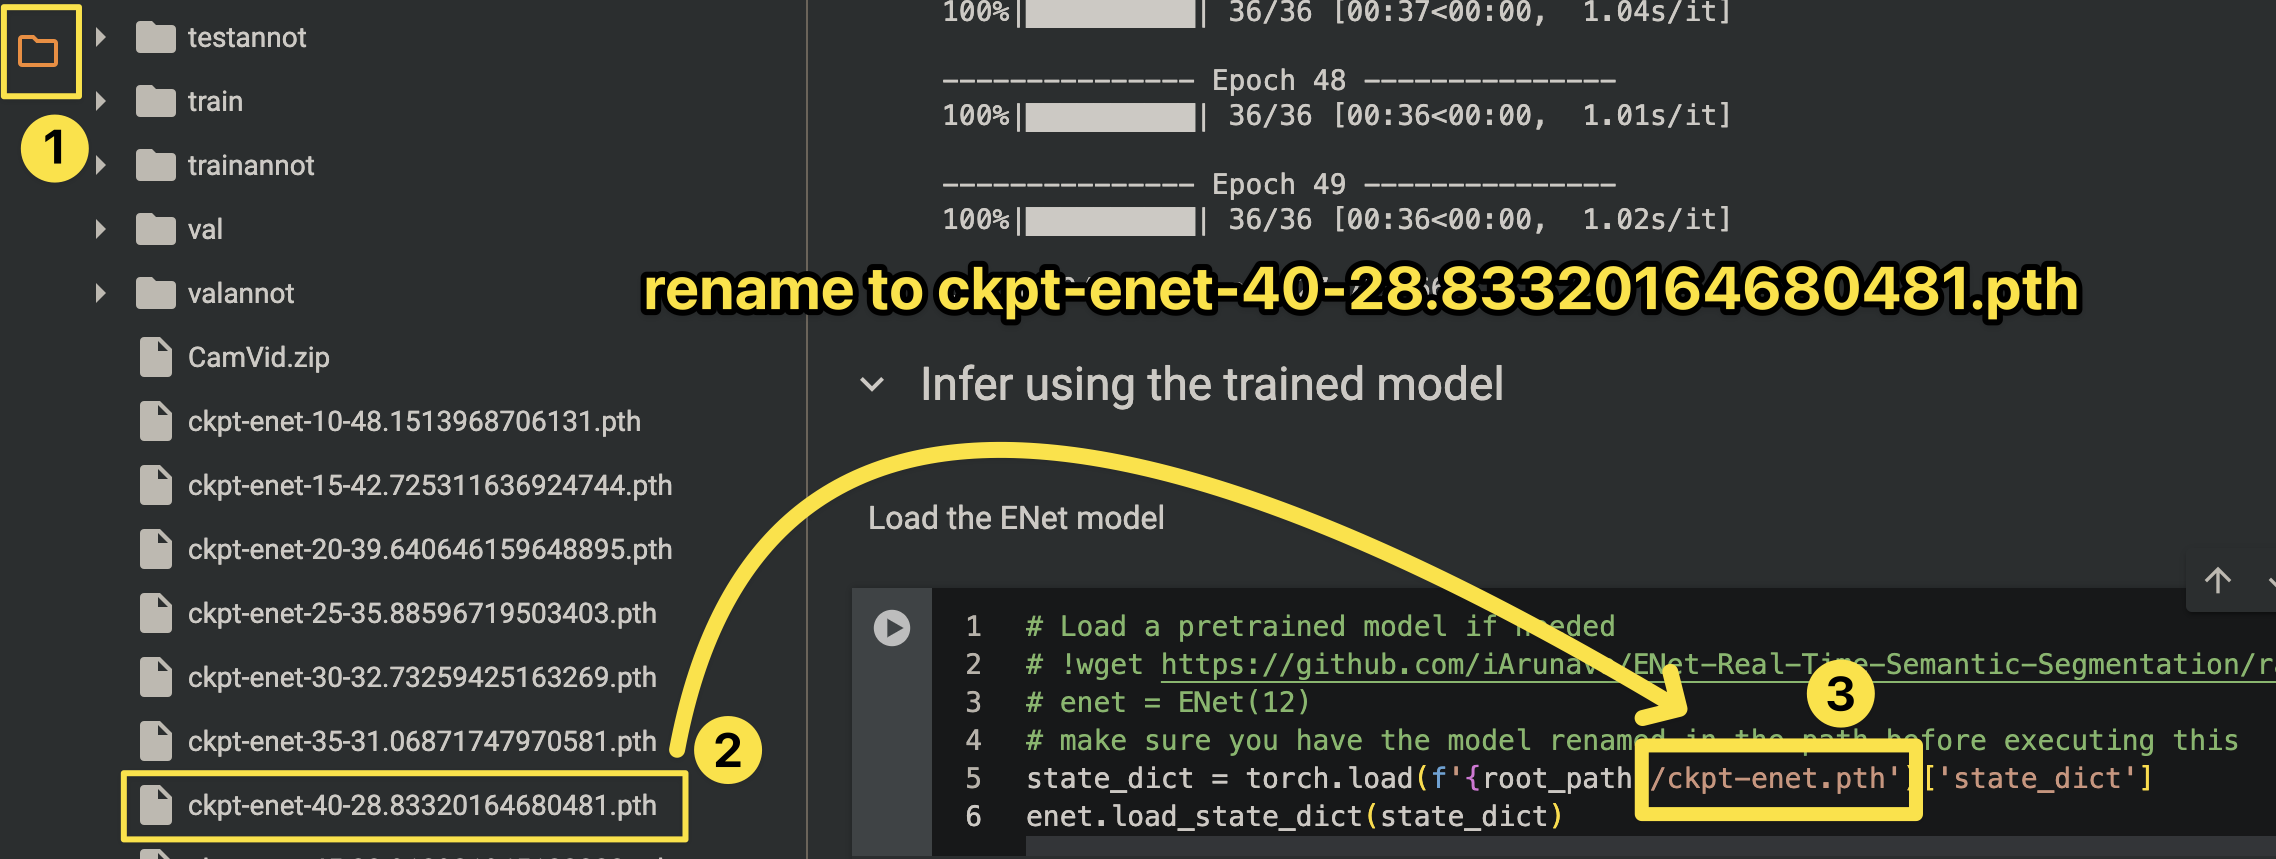
\includegraphics[width=450pt]{assets/enet/camvid/loadenet.png}
    % \caption{SegNet Architecture Diagram}
    \label{fig:using:test2}
\end{figure}

\subsection*{Testing on an image}
\begin{enumerate}
    \item Loading the image: Here you can change the "fname" variable to load the image file from your testing dataset. The code here has been filled with an existing image from the CamVid dataset.
          \begin{lstlisting}
fname = 'Seq05VD_f05100.png'
tmg_ = plt.imread(f'{root_path}/test/' + fname)
tmg_ = cv2.resize(tmg_, (512, 512), cv2.INTER_NEAREST)
tmg = torch.tensor(tmg_).unsqueeze(0).float()
tmg = tmg.transpose(2, 3).transpose(1, 2).to(device)
enet.to(device)
with torch.no_grad():
    out1 = enet(tmg.float()).squeeze(0)
\end{lstlisting}
    \item Generating the class label representation: Execute the following cells in the respective section to generate a label plot for the testing image
          \begin{lstlisting}
smg_ = Image.open(f'{root_path}/testannot/' + fname)
smg_ = cv2.resize(np.array(smg_), (512, 512), cv2.INTER_NEAREST)

mno = 8 # Should be between 0 - n-1 | where n is the number of classes

figure = plt.figure(figsize=(20, 10))
plt.subplot(1, 3, 1)
plt.title('Input Image')
plt.axis('off')
plt.imshow(tmg_)
plt.subplot(1, 3, 2)
plt.title('Output Image')
plt.axis('off')
plt.imshow(out2[mno, :, :])
plt.show()
\end{lstlisting}
          % The following are some of the outputs generated during testing.
          \begin{figure}[H]
              \centering
              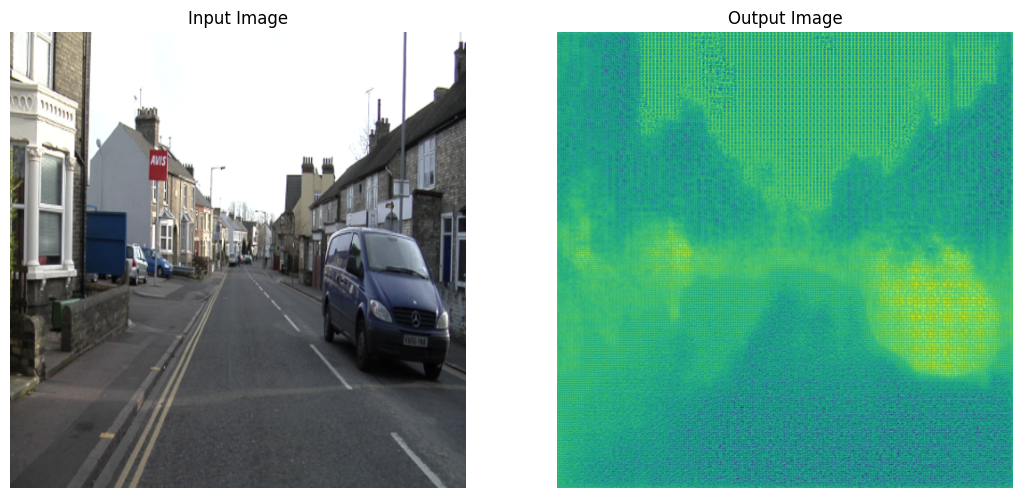
\includegraphics[width=450pt]{assets/enet/camvid/output1.png}
              \caption{Image segmentation was noticeable but far from perfect.}
              \label{fig:using:test5}
          \end{figure}
          %   \begin{figure}[H]
          %       \centering
          %       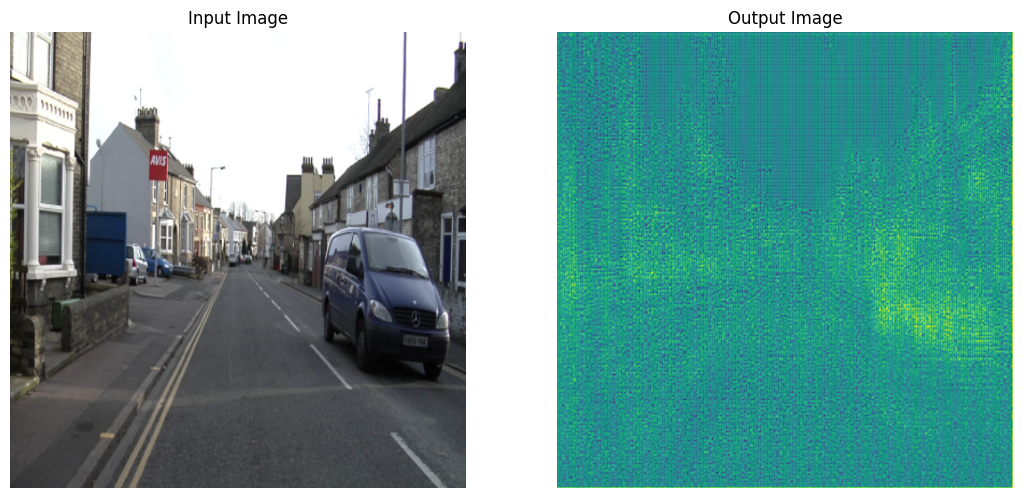
\includegraphics[width=450pt]{assets/enet/camvid/output1alt.png}
          %       \caption{Unexpected results during a testing stage done at a later date}
          %       \label{fig:using:test3}
          %   \end{figure}
    \item Color mapping and decoding: Executing the following code generates the segmented image and shows the ground truth which was already prepared to compare and observe the performance of the trained model.
          \begin{lstlisting}
b_ = out1.data.max(0)[1].cpu().numpy()

def decode_segmap(image):
    Sky = [128, 128, 128]
    Building = [128, 0, 0]
    Pole = [192, 192, 128]
    Road_marking = [255, 69, 0]
    Road = [128, 64, 128]
    Pavement = [60, 40, 222]
    Tree = [128, 128, 0]
    SignSymbol = [192, 128, 128]
    Fence = [64, 64, 128]
    Car = [64, 0, 128]
    Pedestrian = [64, 64, 0]
    Bicyclist = [0, 128, 192]

    label_colours = np.array([Sky, Building, Pole, Road_marking, Road,
                              Pavement, Tree, SignSymbol, Fence, Car,
                              Pedestrian, Bicyclist]).astype(np.uint8)
    r = np.zeros_like(image).astype(np.uint8)
    g = np.zeros_like(image).astype(np.uint8)
    b = np.zeros_like(image).astype(np.uint8)
    for l in range(0, 12):
        r[image == l] = label_colours[l, 0]
        g[image == l] = label_colours[l, 1]
        b[image == l] = label_colours[l, 2]

    rgb = np.zeros((image.shape[0], image.shape[1], 3)).astype(np.uint8)
    rgb[:, :, 0] = b
    rgb[:, :, 1] = g
    rgb[:, :, 2] = r
    return rgb

# decoding the images
true_seg = decode_segmap(smg_)
pred_seg = decode_segmap(b_)

figure = plt.figure(figsize=(20, 10))
plt.subplot(1, 3, 1)
plt.title('Input Image')
plt.axis('off')
plt.imshow(tmg_)
plt.subplot(1, 3, 2)
plt.title('Predicted Segmentation')
plt.axis('off')
plt.imshow(pred_seg)
plt.subplot(1, 3, 3)
plt.title('Ground Truth')
plt.axis('off')
plt.imshow(true_seg)
plt.show()
\end{lstlisting}
          % The following outputs were some samples from the testing done.
          \begin{figure}[H]
              \centering
              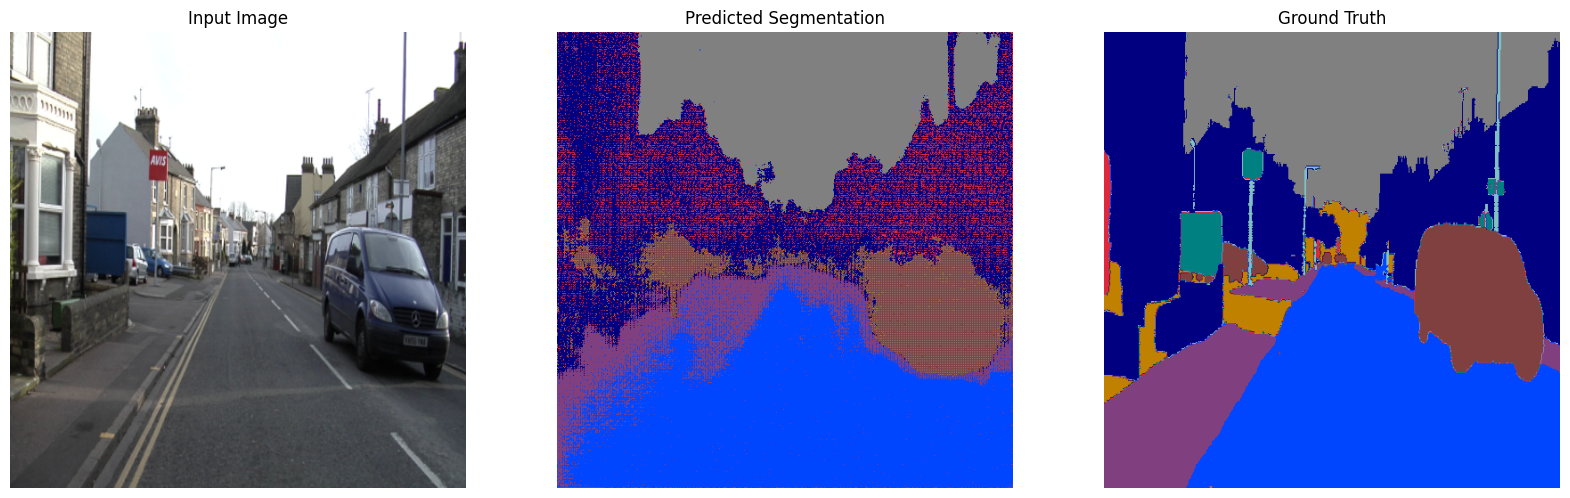
\includegraphics[width=450pt]{assets/enet/camvid/out1.png}
              \caption{The initial test results were promising after a training session with 100 iterations}
              \label{fig:using:test4}
          \end{figure}
          %   \begin{figure}[H]
          %       \centering
          %       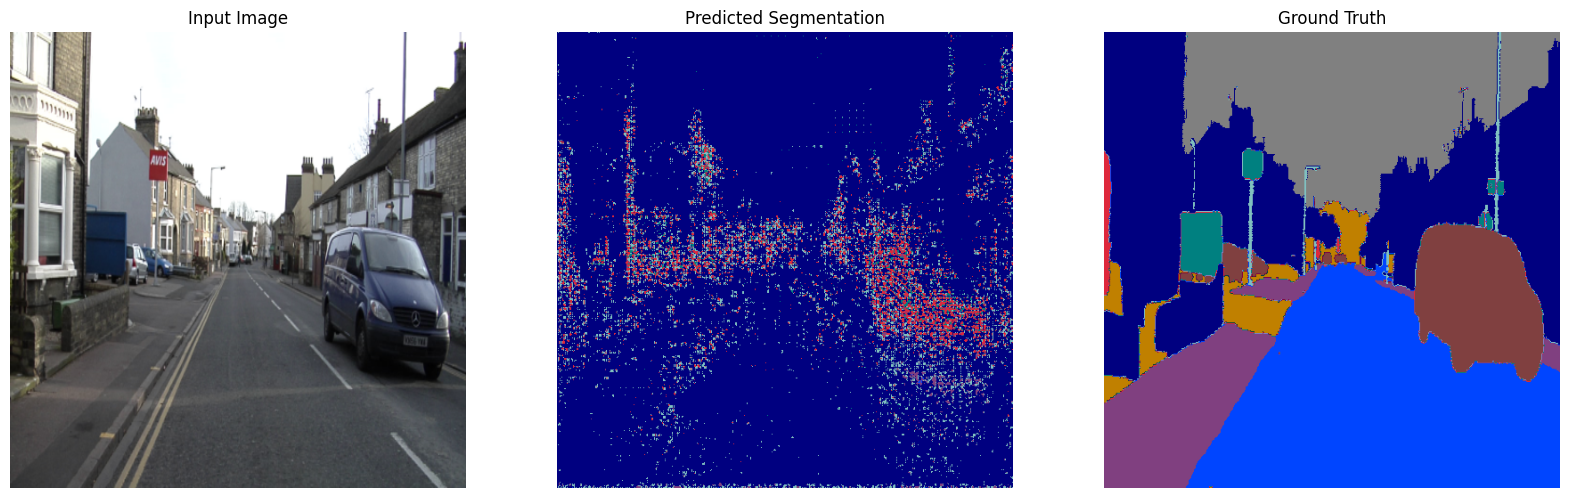
\includegraphics[width=450pt]{assets/enet/camvid/out1alt.png}
          %       \caption{The results were diminished in quality during another testing session with 100 iterations}
          %       \label{fig:using:test6}
          %   \end{figure}
\end{enumerate}



\subsection*{Saving the model and or checkpoints}
When there is a noticeable improvement observed, it is always a good idea to save the relevant parameters and model. The following code will help to save the relevant model to the root directory while also saving the parameter file in the Pytorch format which can then be used to do testing or for deployment or can be converted into a required format for improvement in other platforms. Any file in the Google Colab can be downloaded by navigating to the file directory as mentioned before and right clicking on the relevant file and clicking download.
\begin{lstlisting}
# Save the parameters
checkpoint = {
    'epochs' : e,
    'state_dict' : enet.state_dict()
}
torch.save(checkpoint, f'{root_path}/ckpt-enet-1.pth')
# Save the model
torch.save(enet, f'{root_path}/model.pt')
\end{lstlisting}

\subsection{Engineering Principles followed during the Implementation}
\begin{description}
    \item[Model Optimization:] The model leverages techniques like dimensionality reduction through bottleneck projections, parameter sharing through parallel dilated convolutions, and compact encoder-decoder topology to reduce computational complexity.
    \item[Hardware Acceleration:] By implementing the model in PyTorch and running it on Google Colab, we can take advantage of hardware acceleration through CUDA and cuDNN libraries on NVIDIA GPUs provided by Google's cloud infrastructure.
    \item[Data Parallelism:] The training loop is parallelized across multiple batches through PyTorch's DataLoader abstraction, enabling efficient utilization of the available GPU memory.
    \item[Checkpointing:] The training process supports periodic checkpointing of model weights, allowing training to be resumed from a saved state in case of interruptions or failures.
    \item[Modular Design:] The model implementation is structured into reusable components like bottleneck modules, making it easier to experiment with architectural variations or adapt the codebase for different tasks.
    \item[Visualization:] The notebook includes code for visualizing input images, ground truth segmentation masks, and model predictions, facilitating debugging and qualitative evaluation of results.
\end{description}

This implementation was possible within a short time because of the incredible work done on this existing Pytorch implementation [4] by user iArunava and the notebooks from Kaggle by ajax0564 [1], Davidtvs' repo on Pytorch implementation of ENet [3] were also referred to get more understanding.

With the initial steps completed successfully, we have achieved the first two objectives of obtaining the required datasets and implementing the ENet architecture faithfully in PyTorch. The subsequent goals involve training the model using the prescribed techniques, evaluating its performance against benchmarks, assessing inference speed on embedded hardware if viable, and ultimately comparing the results to existing models like SegNet. By methodically following the outlined plan, we aim to leverage ENet's computational efficiency to develop a reliable and lightweight semantic segmentation model tailored for deployment in resource-constrained industrial environments. Proceeding with the remaining objectives, we will meticulously train, optimize and validate the ENet implementation, culminating in a thorough analysis of its real-world applicability for our box identification task.